\subsection{DATOS}
Amplificador Operacional LM324.

$Vcc = 10V$  $Vss = -10V$

$R1 = 100\Omega$; $R2 = 10K\Omega$; $R3 = 1K\Omega$ y $R4 = 100K\Omega$

\begin{center}
	\resizebox{12cm}{!}{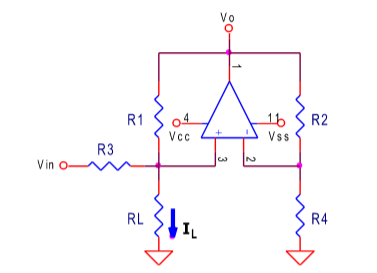
\includegraphics{Imagenes/CII.png}} \\
	\stepcounter{figure}
	\begin{center}
    	\begin{small}
        \textit{Fig.\thefigure \ - \ 	Circuito II: Fuente de corriente controlada por tensión.}
		\end{small}
    \end{center}
\end{center}

\subsection{PARÁMETROS/RELACIONES A ANALIZAR:}


\begin{enumerate}[2.1]
    \item $I_{RL} = f(R_{L} ,V_{IN} ) $; $V_{o} = f(V_{IN} ,R_{L} )$; $R_{Lmax} =f(V_{IN})$
    \item Complete la siguiente tabla con Mediciones/Simulaciones
\end{enumerate}

\begin{table}[H]
\begin{center}
    
\begin{tabular}{|c|l|l|l|l|}
\hline
\multicolumn{2}{|l|}{\multirow{2}{*}{$I_{RL}$}}           & \multicolumn{3}{l|}{$V_{in}[V]$}\\ \cline{3-5} 
\multicolumn{2}{|l|}{}                                     & 0.5          & -1         & 2         \\ \hline
\multirow{5}{*}{$R_{L}[\Omega]$} & 0   &              &            &           \\ \cline{2-5} 
                                                     & 1K  &              &            &           \\ \cline{2-5} 
                                                     & 2K  &              &            &           \\ \cline{2-5} 
                                                     & 5K  &              &            &           \\ \cline{2-5} 
                                                     & 10K &              &            &           \\ \hline
\end{tabular}
\end{center}

\end{table}